\begin{figure}[h]
\centering
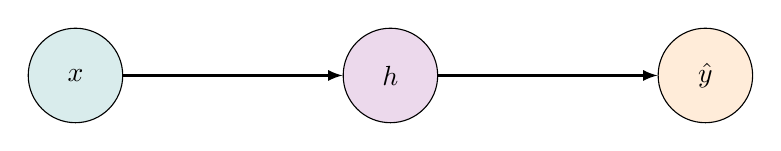
\begin{tikzpicture}[
    neuron/.style={circle, draw, minimum size=1.2cm, align=center},
    input/.style={neuron, fill=teal!15},
    hidden/.style={neuron, fill=violet!15},
    output/.style={neuron, fill=orange!15},
    arrow/.style={-latex, thick}
]

\node[input]  (x) at (0, 0)   {$x$};
\node[hidden] (h) at (4, 0)   {$h$};
\node[output] (y) at (8, 0)   {$\hat{y}$};

\draw[arrow] (x) -- (h);
\draw[arrow] (h) -- (y);

% Layer labels
% \node[below=0.3cm of x] {\small Input layer};
% \node[below=0.3cm of h] {\small Hidden layer};
% \node[below=0.3cm of y] {\small Output layer};

\end{tikzpicture}
\caption{A minimal neural network.}
\label{fig:neural_network}
\end{figure}
